%
% chi.tex -- charakteristische Funktion
%
% (c) \b9 Prof Dr Andreas Müller, Hochschule Rapperswil
%
\documentclass[tikz]{standalone}
\usepackage{amsmath}
\usepackage{times}
\usepackage{txfonts}
\usepackage{pgfplots}
\usepackage{csvsimple}
\usetikzlibrary{arrows,intersections,math}
\begin{document}
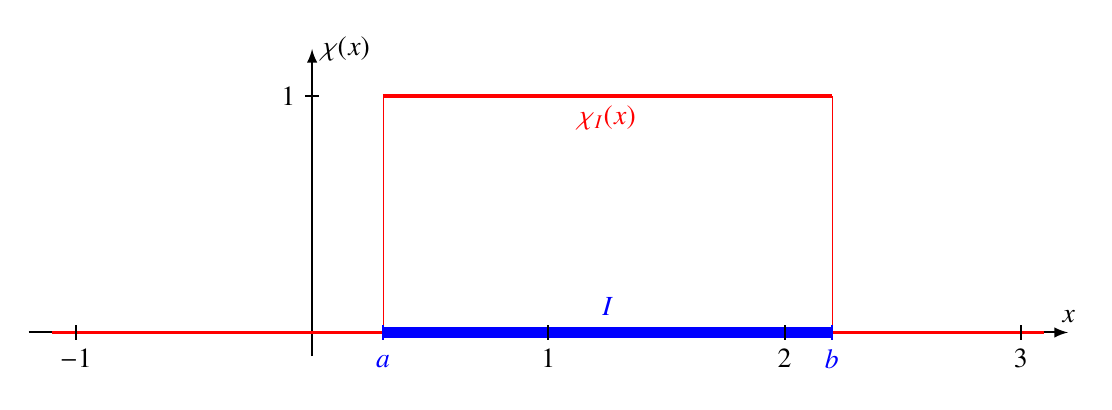
\begin{tikzpicture}[>=latex,scale=3]

\def\s{0.03}
\def\a{0.3}
\def\b{2.2}

\draw[->,line width=0.7pt] (-1.2,0)--(3.2,0) coordinate[label={$x$}];
\draw[->,line width=0.7pt] (0,-0.1)--(0,1.2) coordinate[label={right:$\chi(x)$}];

\draw[color=blue,line width=4pt] (\a,0)--(\b,0);
\node[color=blue] at ({0.5*(\a+\b)},\s) [above] {$I$};

\draw[color=red,line width=1.4pt] (-1.1,0)--(\a,0);
\draw[color=red,line width=0.1pt] (\a,0)--(\a,1);
\draw[color=red,line width=1.4pt] (\a,1)--(\b,1);
\draw[color=red,line width=0.1pt] (\b,1)--(\b,0);
\draw[color=red,line width=1.4pt] (\b,0)--(3.1,0);

\node[color=red] at ({0.5*(\a+\b)},1) [below] {$\chi_I(x)$};

\draw[line width=0.7pt] (-\s,1)--(\s,1);
\node at (-\s,1) [left] {$1$};

\draw[line width=0.7pt,color=blue] (\a,-\s)--(\a,\s);
\draw[line width=0.7pt,color=blue] (\b,-\s)--(\b,\s);

\draw[line width=0.7pt] (-1,-\s)--(-1,\s);
\node at (-1,-\s) [below] {$-1$};
\draw[line width=0.7pt] (1,-\s)--(1,\s);
\node at (1,-\s) [below] {$1$};
\draw[line width=0.7pt] (2,-\s)--(2,\s);
\node at (2,-\s) [below] {$2$};
\draw[line width=0.7pt] (3,-\s)--(3,\s);
\node at (3,-\s) [below] {$3$};

\node[color=blue] at (\a,-\s) [below] {$\mathstrut a$};
\node[color=blue] at (\b,-\s) [below] {$\mathstrut b$};

\end{tikzpicture}
\end{document}

